\documentclass[11pt,compress,t,notes=noshow, xcolor=table]{beamer}
\usepackage[]{graphicx}\usepackage[]{color}
% maxwidth is the original width if it is less than linewidth
% otherwise use linewidth (to make sure the graphics do not exceed the margin)
\makeatletter
\def\maxwidth{ %
  \ifdim\Gin@nat@width>\linewidth
    \linewidth
  \else
    \Gin@nat@width
  \fi
}
\makeatother

\definecolor{fgcolor}{rgb}{0.345, 0.345, 0.345}
\newcommand{\hlnum}[1]{\textcolor[rgb]{0.686,0.059,0.569}{#1}}%
\newcommand{\hlstr}[1]{\textcolor[rgb]{0.192,0.494,0.8}{#1}}%
\newcommand{\hlcom}[1]{\textcolor[rgb]{0.678,0.584,0.686}{\textit{#1}}}%
\newcommand{\hlopt}[1]{\textcolor[rgb]{0,0,0}{#1}}%
\newcommand{\hlstd}[1]{\textcolor[rgb]{0.345,0.345,0.345}{#1}}%
\newcommand{\hlkwa}[1]{\textcolor[rgb]{0.161,0.373,0.58}{\textbf{#1}}}%
\newcommand{\hlkwb}[1]{\textcolor[rgb]{0.69,0.353,0.396}{#1}}%
\newcommand{\hlkwc}[1]{\textcolor[rgb]{0.333,0.667,0.333}{#1}}%
\newcommand{\hlkwd}[1]{\textcolor[rgb]{0.737,0.353,0.396}{\textbf{#1}}}%
\let\hlipl\hlkwb

\usepackage{framed}
\makeatletter
\newenvironment{kframe}{%
 \def\at@end@of@kframe{}%
 \ifinner\ifhmode%
  \def\at@end@of@kframe{\end{minipage}}%
  \begin{minipage}{\columnwidth}%
 \fi\fi%
 \def\FrameCommand##1{\hskip\@totalleftmargin \hskip-\fboxsep
 \colorbox{shadecolor}{##1}\hskip-\fboxsep
     % There is no \\@totalrightmargin, so:
     \hskip-\linewidth \hskip-\@totalleftmargin \hskip\columnwidth}%
 \MakeFramed {\advance\hsize-\width
   \@totalleftmargin\z@ \linewidth\hsize
   \@setminipage}}%
 {\par\unskip\endMakeFramed%
 \at@end@of@kframe}
\makeatother

\definecolor{shadecolor}{rgb}{.97, .97, .97}
\definecolor{messagecolor}{rgb}{0, 0, 0}
\definecolor{warningcolor}{rgb}{1, 0, 1}
\definecolor{errorcolor}{rgb}{1, 0, 0}
\newenvironment{knitrout}{}{} % an empty environment to be redefined in TeX

\usepackage{alltt}
\newcommand{\SweaveOpts}[1]{}  % do not interfere with LaTeX
\newcommand{\SweaveInput}[1]{} % because they are not real TeX commands
\newcommand{\Sexpr}[1]{}       % will only be parsed by R
\newcommand{\xmark}{\ding{55}}%


\usepackage[english]{babel}
\usepackage[utf8]{inputenc}

\usepackage{dsfont}
\usepackage{verbatim}
\usepackage{amsmath}
\usepackage{amsfonts}
\usepackage{amssymb}
\usepackage{bm}
\usepackage{csquotes}
\usepackage{multirow}
\usepackage{longtable}
\usepackage{booktabs}
\usepackage{enumerate}
\usepackage[absolute,overlay]{textpos}
\usepackage{psfrag}
\usepackage{algorithm}
\usepackage{algpseudocode}
\usepackage{eqnarray}
\usepackage{arydshln}
\usepackage{tabularx}
\usepackage{placeins}
\usepackage{tikz}
\usepackage{setspace}
\usepackage{colortbl}
\usepackage{mathtools}
\usepackage{wrapfig}
\usepackage{bm}
\usepackage{amsmath}
\usepackage{pifont}

\usetikzlibrary{shapes,arrows,automata,positioning,calc,chains,trees, shadows}
\tikzset{
  %Define standard arrow tip
  >=stealth',
  %Define style for boxes
  punkt/.style={
    rectangle,
    rounded corners,
    draw=black, very thick,
    text width=6.5em,
    minimum height=2em,
    text centered},
  % Define arrow style
  pil/.style={
    ->,
    thick,
    shorten <=2pt,
    shorten >=2pt,}
}

\usepackage{subfig}

% Defines macros and environments
\usepackage{../../style/lmu-lecture}


\let\code=\texttt
\let\proglang=\textsf

\setkeys{Gin}{width=0.9\textwidth}

\setbeamertemplate{frametitle}{\expandafter\uppercase\expandafter\insertframetitle}

\usepackage{bbm}
% basic latex stuff
\newcommand{\pkg}[1]{{\fontseries{b}\selectfont #1}} %fontstyle for R packages
\newcommand{\lz}{\vspace{0.5cm}} %vertical space
\newcommand{\dlz}{\vspace{1cm}} %double vertical space
\newcommand{\oneliner}[1] % Oneliner for important statements
{\begin{block}{}\begin{center}\begin{Large}#1\end{Large}\end{center}\end{block}}


%new environments
\newenvironment{vbframe}  %frame with breaks and verbatim
{
 \begin{frame}[containsverbatim,allowframebreaks]
}
{
\end{frame}
}

\newenvironment{vframe}  %frame with verbatim without breaks (to avoid numbering one slided frames)
{
 \begin{frame}[containsverbatim]
}
{
\end{frame}
}

\newenvironment{blocki}[1]   % itemize block
{
 \begin{block}{#1}\begin{itemize}
}
{
\end{itemize}\end{block}
}

\newenvironment{fragileframe}[2]{  %fragile frame with framebreaks
\begin{frame}[allowframebreaks, fragile, environment = fragileframe]
\frametitle{#1}
#2}
{\end{frame}}


\newcommand{\myframe}[2]{  %short for frame with framebreaks
\begin{frame}[allowframebreaks]
\frametitle{#1}
#2
\end{frame}}

\newcommand{\remark}[1]{
  \textbf{Remark:} #1
}

\newcommand{\citebutton}[2]{%
\NoCaseChange{\resizebox{!}{9pt}{\protect\beamergotobutton{\href{#2}{#1}}}}%
}



\newenvironment{deleteframe}
{
\begingroup
\usebackgroundtemplate{\includegraphics[width=\paperwidth,height=\paperheight]{../style/color/red.png}}
 \begin{frame}
}
{
\end{frame}
\endgroup
}
\newenvironment{simplifyframe}
{
\begingroup
\usebackgroundtemplate{\includegraphics[width=\paperwidth,height=\paperheight]{../style/color/yellow.png}}
 \begin{frame}
}
{
\end{frame}
\endgroup
}\newenvironment{draftframe}
{
\begingroup
\usebackgroundtemplate{\includegraphics[width=\paperwidth,height=\paperheight]{../style/color/green.jpg}}
 \begin{frame}
}
{
\end{frame}
\endgroup
}
% https://tex.stackexchange.com/a/261480: textcolor that works in mathmode
\makeatletter
\renewcommand*{\@textcolor}[3]{%
  \protect\leavevmode
  \begingroup
    \color#1{#2}#3%
  \endgroup
}
\makeatother





% math spaces
\ifdefined\N                                                                
\renewcommand{\N}{\mathds{N}} % N, naturals
\else \newcommand{\N}{\mathds{N}} \fi 
\newcommand{\Z}{\mathds{Z}} % Z, integers
\newcommand{\Q}{\mathds{Q}} % Q, rationals
\newcommand{\R}{\mathds{R}} % R, reals
\ifdefined\C 
  \renewcommand{\C}{\mathds{C}} % C, complex
\else \newcommand{\C}{\mathds{C}} \fi
\newcommand{\continuous}{\mathcal{C}} % C, space of continuous functions
\newcommand{\M}{\mathcal{M}} % machine numbers
\newcommand{\epsm}{\epsilon_m} % maximum error

% counting / finite sets
\newcommand{\setzo}{\{0, 1\}} % set 0, 1
\newcommand{\setmp}{\{-1, +1\}} % set -1, 1
\newcommand{\unitint}{[0, 1]} % unit interval

% basic math stuff
\newcommand{\xt}{\tilde x} % x tilde
\newcommand{\argmax}{\operatorname{arg\,max}} % argmax
\newcommand{\argmin}{\operatorname{arg\,min}} % argmin
\newcommand{\argminlim}{\mathop{\mathrm{arg\,min}}\limits} % argmax with limits
\newcommand{\argmaxlim}{\mathop{\mathrm{arg\,max}}\limits} % argmin with limits  
\newcommand{\sign}{\operatorname{sign}} % sign, signum
\newcommand{\I}{\mathbb{I}} % I, indicator
\newcommand{\order}{\mathcal{O}} % O, order
\newcommand{\pd}[2]{\frac{\partial{#1}}{\partial #2}} % partial derivative
\newcommand{\floorlr}[1]{\left\lfloor #1 \right\rfloor} % floor
\newcommand{\ceillr}[1]{\left\lceil #1 \right\rceil} % ceiling

% sums and products
\newcommand{\sumin}{\sum\limits_{i=1}^n} % summation from i=1 to n
\newcommand{\sumim}{\sum\limits_{i=1}^m} % summation from i=1 to m
\newcommand{\sumjn}{\sum\limits_{j=1}^n} % summation from j=1 to p
\newcommand{\sumjp}{\sum\limits_{j=1}^p} % summation from j=1 to p
\newcommand{\sumik}{\sum\limits_{i=1}^k} % summation from i=1 to k
\newcommand{\sumkg}{\sum\limits_{k=1}^g} % summation from k=1 to g
\newcommand{\sumjg}{\sum\limits_{j=1}^g} % summation from j=1 to g
\newcommand{\meanin}{\frac{1}{n} \sum\limits_{i=1}^n} % mean from i=1 to n
\newcommand{\meanim}{\frac{1}{m} \sum\limits_{i=1}^m} % mean from i=1 to n
\newcommand{\meankg}{\frac{1}{g} \sum\limits_{k=1}^g} % mean from k=1 to g
\newcommand{\prodin}{\prod\limits_{i=1}^n} % product from i=1 to n
\newcommand{\prodkg}{\prod\limits_{k=1}^g} % product from k=1 to g
\newcommand{\prodjp}{\prod\limits_{j=1}^p} % product from j=1 to p

% linear algebra
\newcommand{\one}{\boldsymbol{1}} % 1, unitvector
\newcommand{\zero}{\mathbf{0}} % 0-vector
\newcommand{\id}{\boldsymbol{I}} % I, identity
\newcommand{\diag}{\operatorname{diag}} % diag, diagonal
\newcommand{\trace}{\operatorname{tr}} % tr, trace
\newcommand{\spn}{\operatorname{span}} % span
\newcommand{\scp}[2]{\left\langle #1, #2 \right\rangle} % <.,.>, scalarproduct
\newcommand{\mat}[1]{\begin{pmatrix} #1 \end{pmatrix}} % short pmatrix command
\newcommand{\Amat}{\mathbf{A}} % matrix A
\newcommand{\Deltab}{\mathbf{\Delta}} % error term for vectors

% basic probability + stats
\renewcommand{\P}{\mathds{P}} % P, probability
\newcommand{\E}{\mathds{E}} % E, expectation
\newcommand{\var}{\mathsf{Var}} % Var, variance
\newcommand{\cov}{\mathsf{Cov}} % Cov, covariance
\newcommand{\corr}{\mathsf{Corr}} % Corr, correlation
\newcommand{\normal}{\mathcal{N}} % N of the normal distribution
\newcommand{\iid}{\overset{i.i.d}{\sim}} % dist with i.i.d superscript
\newcommand{\distas}[1]{\overset{#1}{\sim}} % ... is distributed as ...

% machine learning
\newcommand{\Xspace}{\mathcal{X}} % X, input space
\newcommand{\Yspace}{\mathcal{Y}} % Y, output space
\newcommand{\nset}{\{1, \ldots, n\}} % set from 1 to n
\newcommand{\pset}{\{1, \ldots, p\}} % set from 1 to p
\newcommand{\gset}{\{1, \ldots, g\}} % set from 1 to g
\newcommand{\Pxy}{\mathbb{P}_{xy}} % P_xy
\newcommand{\Exy}{\mathbb{E}_{xy}} % E_xy: Expectation over random variables xy
\newcommand{\xv}{\mathbf{x}} % vector x (bold)
\newcommand{\xtil}{\tilde{\mathbf{x}}} % vector x-tilde (bold)
\newcommand{\yv}{\mathbf{y}} % vector y (bold)
\newcommand{\xy}{(\xv, y)} % observation (x, y)
\newcommand{\xvec}{\left(x_1, \ldots, x_p\right)^\top} % (x1, ..., xp) 
\newcommand{\Xmat}{\mathbf{X}} % Design matrix
\newcommand{\allDatasets}{\mathds{D}} % The set of all datasets
\newcommand{\allDatasetsn}{\mathds{D}_n}  % The set of all datasets of size n 
\newcommand{\D}{\mathcal{D}} % D, data
\newcommand{\Dn}{\D_n} % D_n, data of size n
\newcommand{\Dtrain}{\mathcal{D}_{\text{train}}} % D_train, training set
\newcommand{\Dtest}{\mathcal{D}_{\text{test}}} % D_test, test set
\newcommand{\xyi}[1][i]{\left(\xv^{(#1)}, y^{(#1)}\right)} % (x^i, y^i), i-th observation
\newcommand{\Dset}{\left( \xyi[1], \ldots, \xyi[n]\right)} % {(x1,y1)), ..., (xn,yn)}, data
\newcommand{\defAllDatasetsn}{(\Xspace \times \Yspace)^n} % Def. of the set of all datasets of size n 
\newcommand{\defAllDatasets}{\bigcup_{n \in \N}(\Xspace \times \Yspace)^n} % Def. of the set of all datasets 
\newcommand{\xdat}{\left\{ \xv^{(1)}, \ldots, \xv^{(n)}\right\}} % {x1, ..., xn}, input data
\newcommand{\yvec}{\left(y^{(1)}, \hdots, y^{(n)}\right)^\top} % (y1, ..., yn), vector of outcomes
\renewcommand{\xi}[1][i]{\xv^{(#1)}} % x^i, i-th observed value of x
\newcommand{\yi}[1][i]{y^{(#1)}} % y^i, i-th observed value of y 
\newcommand{\xivec}{\left(x^{(i)}_1, \ldots, x^{(i)}_p\right)^\top} % (x1^i, ..., xp^i), i-th observation vector
\newcommand{\xj}{\xv_j} % x_j, j-th feature
\newcommand{\xjvec}{\left(x^{(1)}_j, \ldots, x^{(n)}_j\right)^\top} % (x^1_j, ..., x^n_j), j-th feature vector
\newcommand{\phiv}{\mathbf{\phi}} % Basis transformation function phi
\newcommand{\phixi}{\mathbf{\phi}^{(i)}} % Basis transformation of xi: phi^i := phi(xi)

%%%%%% ml - models general
\newcommand{\lamv}{\bm{\lambda}} % lambda vector, hyperconfiguration vector
\newcommand{\Lam}{\bm{\Lambda}}	 % Lambda, space of all hpos
% Inducer / Inducing algorithm
\newcommand{\preimageInducer}{\left(\defAllDatasets\right)\times\Lam} % Set of all datasets times the hyperparameter space
\newcommand{\preimageInducerShort}{\allDatasets\times\Lam} % Set of all datasets times the hyperparameter space
% Inducer / Inducing algorithm
\newcommand{\ind}{\mathcal{I}} % Inducer, inducing algorithm, learning algorithm 

% continuous prediction function f
\newcommand{\ftrue}{f_{\text{true}}}  % True underlying function (if a statistical model is assumed)
\newcommand{\ftruex}{\ftrue(\xv)} % True underlying function (if a statistical model is assumed)
\newcommand{\fx}{f(\xv)} % f(x), continuous prediction function
\newcommand{\fdomains}{f: \Xspace \rightarrow \R^g} % f with domain and co-domain
\newcommand{\Hspace}{\mathcal{H}} % hypothesis space where f is from
\newcommand{\fbayes}{f^{\ast}} % Bayes-optimal model
\newcommand{\fxbayes}{f^{\ast}(\xv)} % Bayes-optimal model
\newcommand{\fkx}[1][k]{f_{#1}(\xv)} % f_j(x), discriminant component function
\newcommand{\fh}{\hat{f}} % f hat, estimated prediction function
\newcommand{\fxh}{\fh(\xv)} % fhat(x)
\newcommand{\fxt}{f(\xv ~|~ \thetab)} % f(x | theta)
\newcommand{\fxi}{f\left(\xv^{(i)}\right)} % f(x^(i))
\newcommand{\fxih}{\hat{f}\left(\xv^{(i)}\right)} % f(x^(i))
\newcommand{\fxit}{f\left(\xv^{(i)} ~|~ \thetab\right)} % f(x^(i) | theta)
\newcommand{\fhD}{\fh_{\D}} % fhat_D, estimate of f based on D
\newcommand{\fhDtrain}{\fh_{\Dtrain}} % fhat_Dtrain, estimate of f based on D
\newcommand{\fhDnlam}{\fh_{\Dn, \lamv}} %model learned on Dn with hp lambda
\newcommand{\fhDlam}{\fh_{\D, \lamv}} %model learned on D with hp lambda
\newcommand{\fhDnlams}{\fh_{\Dn, \lamv^\ast}} %model learned on Dn with optimal hp lambda 
\newcommand{\fhDlams}{\fh_{\D, \lamv^\ast}} %model learned on D with optimal hp lambda 

% discrete prediction function h
\newcommand{\hx}{h(\xv)} % h(x), discrete prediction function
\newcommand{\hh}{\hat{h}} % h hat
\newcommand{\hxh}{\hat{h}(\xv)} % hhat(x)
\newcommand{\hxt}{h(\xv | \thetab)} % h(x | theta)
\newcommand{\hxi}{h\left(\xi\right)} % h(x^(i))
\newcommand{\hxit}{h\left(\xi ~|~ \thetab\right)} % h(x^(i) | theta)
\newcommand{\hbayes}{h^{\ast}} % Bayes-optimal classification model
\newcommand{\hxbayes}{h^{\ast}(\xv)} % Bayes-optimal classification model

% yhat
\newcommand{\yh}{\hat{y}} % yhat for prediction of target
\newcommand{\yih}{\hat{y}^{(i)}} % yhat^(i) for prediction of ith targiet
\newcommand{\resi}{\yi- \yih}

% theta
\newcommand{\thetah}{\hat{\theta}} % theta hat
\newcommand{\thetab}{\bm{\theta}} % theta vector
\newcommand{\thetabh}{\bm{\hat\theta}} % theta vector hat
\newcommand{\thetat}[1][t]{\thetab^{[#1]}} % theta^[t] in optimization
\newcommand{\thetatn}[1][t]{\thetab^{[#1 +1]}} % theta^[t+1] in optimization
\newcommand{\thetahDnlam}{\thetabh_{\Dn, \lamv}} %theta learned on Dn with hp lambda
\newcommand{\thetahDlam}{\thetabh_{\D, \lamv}} %theta learned on D with hp lambda
\newcommand{\mint}{\min_{\thetab \in \Theta}} % min problem theta
\newcommand{\argmint}{\argmin_{\thetab \in \Theta}} % argmin theta

% densities + probabilities
% pdf of x 
\newcommand{\pdf}{p} % p
\newcommand{\pdfx}{p(\xv)} % p(x)
\newcommand{\pixt}{\pi(\xv~|~ \thetab)} % pi(x|theta), pdf of x given theta
\newcommand{\pixit}{\pi\left(\xi ~|~ \thetab\right)} % pi(x^i|theta), pdf of x given theta
\newcommand{\pixii}{\pi\left(\xi\right)} % pi(x^i), pdf of i-th x 

% pdf of (x, y)
\newcommand{\pdfxy}{p(\xv,y)} % p(x, y)
\newcommand{\pdfxyt}{p(\xv, y ~|~ \thetab)} % p(x, y | theta)
\newcommand{\pdfxyit}{p\left(\xi, \yi ~|~ \thetab\right)} % p(x^(i), y^(i) | theta)

% pdf of x given y
\newcommand{\pdfxyk}[1][k]{p(\xv | y= #1)} % p(x | y = k)
\newcommand{\lpdfxyk}[1][k]{\log p(\xv | y= #1)} % log p(x | y = k)
\newcommand{\pdfxiyk}[1][k]{p\left(\xi | y= #1 \right)} % p(x^i | y = k)

% prior probabilities
\newcommand{\pik}[1][k]{\pi_{#1}} % pi_k, prior
\newcommand{\lpik}[1][k]{\log \pi_{#1}} % log pi_k, log of the prior
\newcommand{\pit}{\pi(\thetab)} % Prior probability of parameter theta

% posterior probabilities
\newcommand{\post}{\P(y = 1 ~|~ \xv)} % P(y = 1 | x), post. prob for y=1
\newcommand{\postk}[1][k]{\P(y = #1 ~|~ \xv)} % P(y = k | y), post. prob for y=k
\newcommand{\pidomains}{\pi: \Xspace \rightarrow \unitint} % pi with domain and co-domain
\newcommand{\pibayes}{\pi^{\ast}} % Bayes-optimal classification model
\newcommand{\pixbayes}{\pi^{\ast}(\xv)} % Bayes-optimal classification model
\newcommand{\pix}{\pi(\xv)} % pi(x), P(y = 1 | x)
\newcommand{\pikx}[1][k]{\pi_{#1}(\xv)} % pi_k(x), P(y = k | x)
\newcommand{\pikxt}[1][k]{\pi_{#1}(\xv ~|~ \thetab)} % pi_k(x | theta), P(y = k | x, theta)
\newcommand{\pixh}{\hat \pi(\xv)} % pi(x) hat, P(y = 1 | x) hat
\newcommand{\pikxh}[1][k]{\hat \pi_{#1}(\xv)} % pi_k(x) hat, P(y = k | x) hat
\newcommand{\pixih}{\hat \pi(\xi)} % pi(x^(i)) with hat
\newcommand{\pikxih}[1][k]{\hat \pi_{#1}(\xi)} % pi_k(x^(i)) with hat
\newcommand{\pdfygxt}{p(y ~|~\xv, \thetab)} % p(y | x, theta)
\newcommand{\pdfyigxit}{p\left(\yi ~|~\xi, \thetab\right)} % p(y^i |x^i, theta)
\newcommand{\lpdfygxt}{\log \pdfygxt } % log p(y | x, theta)
\newcommand{\lpdfyigxit}{\log \pdfyigxit} % log p(y^i |x^i, theta)

% probababilistic
\newcommand{\bayesrulek}[1][k]{\frac{\P(\xv | y= #1) \P(y= #1)}{\P(\xv)}} % Bayes rule
\newcommand{\muk}{\bm{\mu_k}} % mean vector of class-k Gaussian (discr analysis) 

% residual and margin
\newcommand{\eps}{\epsilon} % residual, stochastic
\newcommand{\epsi}{\epsilon^{(i)}} % epsilon^i, residual, stochastic
\newcommand{\epsh}{\hat{\epsilon}} % residual, estimated
\newcommand{\yf}{y \fx} % y f(x), margin
\newcommand{\yfi}{\yi \fxi} % y^i f(x^i), margin
\newcommand{\Sigmah}{\hat \Sigma} % estimated covariance matrix
\newcommand{\Sigmahj}{\hat \Sigma_j} % estimated covariance matrix for the j-th class

% ml - loss, risk, likelihood
\newcommand{\Lyf}{L\left(y, f\right)} % L(y, f), loss function
\newcommand{\Lxy}{L\left(y, \fx\right)} % L(y, f(x)), loss function
\newcommand{\Lxyi}{L\left(\yi, \fxi\right)} % loss of observation
\newcommand{\Lxyt}{L\left(y, \fxt\right)} % loss with f parameterized
\newcommand{\Lxyit}{L\left(\yi, \fxit\right)} % loss of observation with f parameterized
\newcommand{\Lxym}{L\left(\yi, f\left(\bm{\tilde{x}}^{(i)} ~|~ \thetab\right)\right)} % loss of observation with f parameterized
\newcommand{\Lpixy}{L\left(y, \pix\right)} % loss in classification
\newcommand{\Lpixyi}{L\left(\yi, \pixii\right)} % loss of observation in classification
\newcommand{\Lpixyt}{L\left(y, \pixt\right)} % loss with pi parameterized
\newcommand{\Lpixyit}{L\left(\yi, \pixit\right)} % loss of observation with pi parameterized
\newcommand{\Lhxy}{L\left(y, \hx\right)} % L(y, h(x)), loss function on discrete classes
\newcommand{\Lr}{L\left(r\right)} % L(r), loss defined on residual (reg) / margin (classif)
\newcommand{\lone}{|y - \fx|} % L1 loss
\newcommand{\ltwo}{\left(y - \fx\right)^2} % L2 loss
\newcommand{\lbernoullimp}{\ln(1 + \exp(-y \cdot \fx))} % Bernoulli loss for -1, +1 encoding
\newcommand{\lbernoullizo}{- y \cdot \fx + \log(1 + \exp(\fx))} % Bernoulli loss for 0, 1 encoding
\newcommand{\lcrossent}{- y \log \left(\pix\right) - (1 - y) \log \left(1 - \pix\right)} % cross-entropy loss
\newcommand{\lbrier}{\left(\pix - y \right)^2} % Brier score
\newcommand{\risk}{\mathcal{R}} % R, risk
\newcommand{\riskbayes}{\mathcal{R}^\ast}
\newcommand{\riskf}{\risk(f)} % R(f), risk
\newcommand{\riskdef}{\E_{y|\xv}\left(\Lxy \right)} % risk def (expected loss)
\newcommand{\riskt}{\mathcal{R}(\thetab)} % R(theta), risk
\newcommand{\riske}{\mathcal{R}_{\text{emp}}} % R_emp, empirical risk w/o factor 1 / n
\newcommand{\riskeb}{\bar{\mathcal{R}}_{\text{emp}}} % R_emp, empirical risk w/ factor 1 / n
\newcommand{\riskef}{\riske(f)} % R_emp(f)
\newcommand{\risket}{\mathcal{R}_{\text{emp}}(\thetab)} % R_emp(theta)
\newcommand{\riskr}{\mathcal{R}_{\text{reg}}} % R_reg, regularized risk
\newcommand{\riskrt}{\mathcal{R}_{\text{reg}}(\thetab)} % R_reg(theta)
\newcommand{\riskrf}{\riskr(f)} % R_reg(f)
\newcommand{\riskrth}{\hat{\mathcal{R}}_{\text{reg}}(\thetab)} % hat R_reg(theta)
\newcommand{\risketh}{\hat{\mathcal{R}}_{\text{emp}}(\thetab)} % hat R_emp(theta)
\newcommand{\LL}{\mathcal{L}} % L, likelihood
\newcommand{\LLt}{\mathcal{L}(\thetab)} % L(theta), likelihood
\newcommand{\LLtx}{\mathcal{L}(\thetab | \xv)} % L(theta|x), likelihood
\newcommand{\logl}{\ell} % l, log-likelihood
\newcommand{\loglt}{\logl(\thetab)} % l(theta), log-likelihood
\newcommand{\logltx}{\logl(\thetab | \xv)} % l(theta|x), log-likelihood
\newcommand{\errtrain}{\text{err}_{\text{train}}} % training error
\newcommand{\errtest}{\text{err}_{\text{test}}} % test error
\newcommand{\errexp}{\overline{\text{err}_{\text{test}}}} % avg training error

% lm
\newcommand{\thx}{\thetab^\top \xv} % linear model
\newcommand{\olsest}{(\Xmat^\top \Xmat)^{-1} \Xmat^\top \yv} % OLS estimator in LM 


\newcommand{\titlefigure}{figure/fig-title-knn-3d-contour.png}
\newcommand{\learninggoals}{
\item Understand the basic idea of $k$-NN for regression and classification
\item Understand that $k$-NN is a non-parametric, local model
\item Know different distance measures for different scales of feature variables
}


\title{Introduction to Machine Learning}
% \author{Bernd Bischl, Christoph Molnar, Daniel Schalk, Fabian Scheipl}
\institute{\href{https://compstat-lmu.github.io/lecture_i2ml/}{compstat-lmu.github.io/lecture\_i2ml}}
\date{}

\begin{document}
\lecturechapter{$k$-Nearest Neighbors}
\lecture{Introduction to Machine Learning}

% \begin{vbframe}{Nearest Neighbors: Intuition}
% 
% \begin{itemize}
%  \item Say we know locations of cities in 2 different countries.
%  \item Say we know which city is in which country.
%  \item Say we don't know where the countries' border is.
%  \item For a given location, we want to figure out which country it belongs to.
%  \item Nearest neighbor rule: every location belongs to the same country as the closest city.
%  \item $k$-nearest neighbor rule: vote over the $k$ closest cities (smoother)
% \end{itemize}
% %\begin{center}
% %  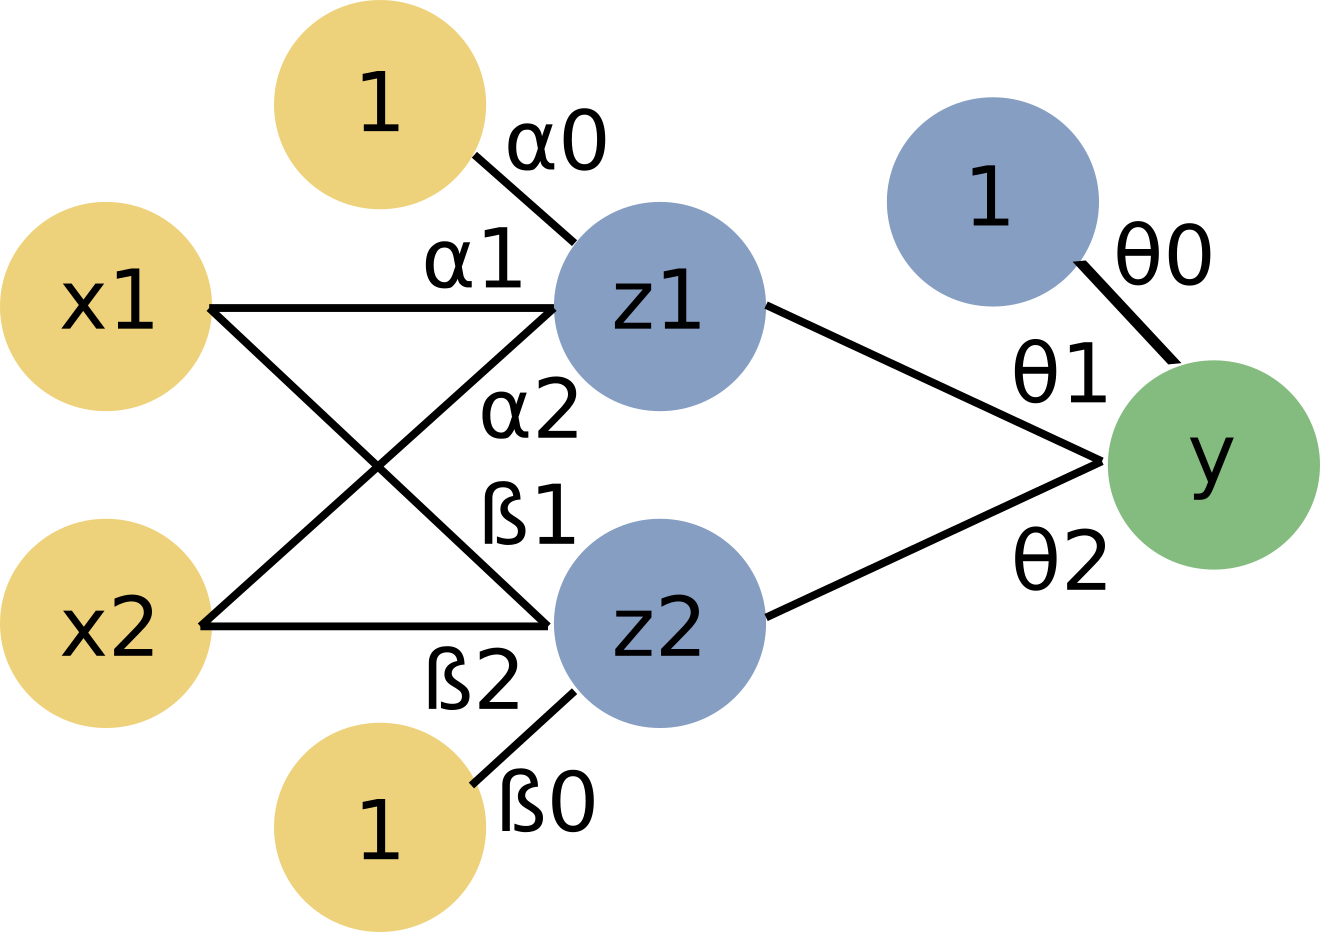
\includegraphics[width=.5\textwidth]{figure_man/nn.png}
% %\end{center}
% \end{vbframe}



\begin{vbframe}{$k$-Nearest-Neighbors}

\begin{itemize}
\item $k$-\textbf{NN} can be used for regression and classification.
\item Generates "similar" predictions for $\xv$ to its $k$ closest neighbors.
\item "Closeness" requires a distance or similarity measure.
\item The set containing the $k$ closest points $\xi$ to $\xv$ in the training data is called  the $k$-\textbf{neighborhood} $N_k(\xv)$ of $\xv$.
\end{itemize}


\begin{knitrout}\scriptsize
\definecolor{shadecolor}{rgb}{0.969, 0.969, 0.969}\color{fgcolor}

{\centering 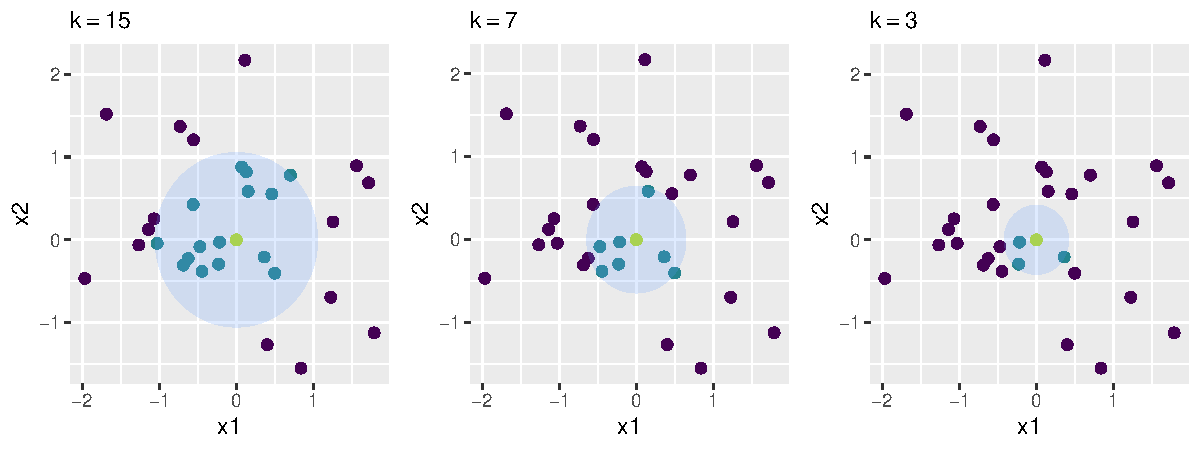
\includegraphics[width=0.95\textwidth]{figure/reg_knn_1} 

}



\end{knitrout}

\end{vbframe}



    %\item It is based on a special case of the $L_p$-norm: $||x||_p = (|x_1|^p + ... + |x_q|^p)^\frac{1}{p}$ with $p = 2$
    
% \framebreak
% \item Example:
% \begin{itemize}
%   \item Three data points with two metric features each: $a = (1, 3),
%   b = (4, 5)$ and $c = (7, 8)$
%   \item Which is the nearest neighbor of $b$ in terms of the Euclidean distance?
%   \item $d(b, a) = \sqrt{(4 - 1)^2 + (5 - 3)^2} = 3.61$
%   \item $d(b, c) = \sqrt{(4 - 7)^2 + (5 - 8)^2} = 4.24$
%   \item $\Rightarrow a$ is the nearest neighbor for $b$.
% \end{itemize}
%     \item Alternative distance measures are:
%     \begin{itemize}
%       \item Manhattan distance% based on the $L_1$-norm:
%         \begin{equation*}
%           d_{manhattan}(\xv, \tilde{\xv}) = \sumjp |x_j - \tilde{x}_j|
%         \end{equation*}
%       \item Mahalanobis distance (takes covariances in $\Xspace$ into account)
%     \end{itemize}
%   \end{itemize}

% \framebreak
% 
% Comparison between Euclidean and Manhattan distance measures:\\
\begin{vbframe}{Distance Measures}





  
  
% \textbf{How to calculate distances?}
\begin{itemize}
  \item Popular for numerical features: \textbf{Minkowski} distances
  of the form $\| \xv - \tilde \xv \|_q = \left( \sumjp |x_j - \tilde x_j|^q 
  \right)^{\frac{1}{q}}$ for $\xv, \tilde{\xv} \in \Xspace$ with $p$ numeric 
  features
  \item Especially, \textbf{Manhattan} ($q = 1$) and \textbf{Euclidean} 
  ($q = 2$) distance 
\end{itemize}

\vspace{0.3cm}

\begin{minipage}{0.42\textwidth}
  \begin{itemize}
    \small
    \item[] $d_{Manhattan}\left(\xv, \tilde{\xv}\right) = \| \xv - 
    \tilde \xv \|_1$ \\
    $=\sumjp |x_j - \tilde{x}_j| $
    \item[]
    \item[] $d_{Euclidean}\left(\xv, \tilde{\xv}\right) = \| \xv - 
    \tilde \xv \|_2$ \\
    \vspace{0.1cm}
    $= \sqrt{\sumjp(x_j- \tilde{x}_j)^2}$
  \end {itemize}
\end{minipage}%
\begin{minipage}{0.58\textwidth}
 %\strut\vspace*{-\baselineskip}\newline
 \centering 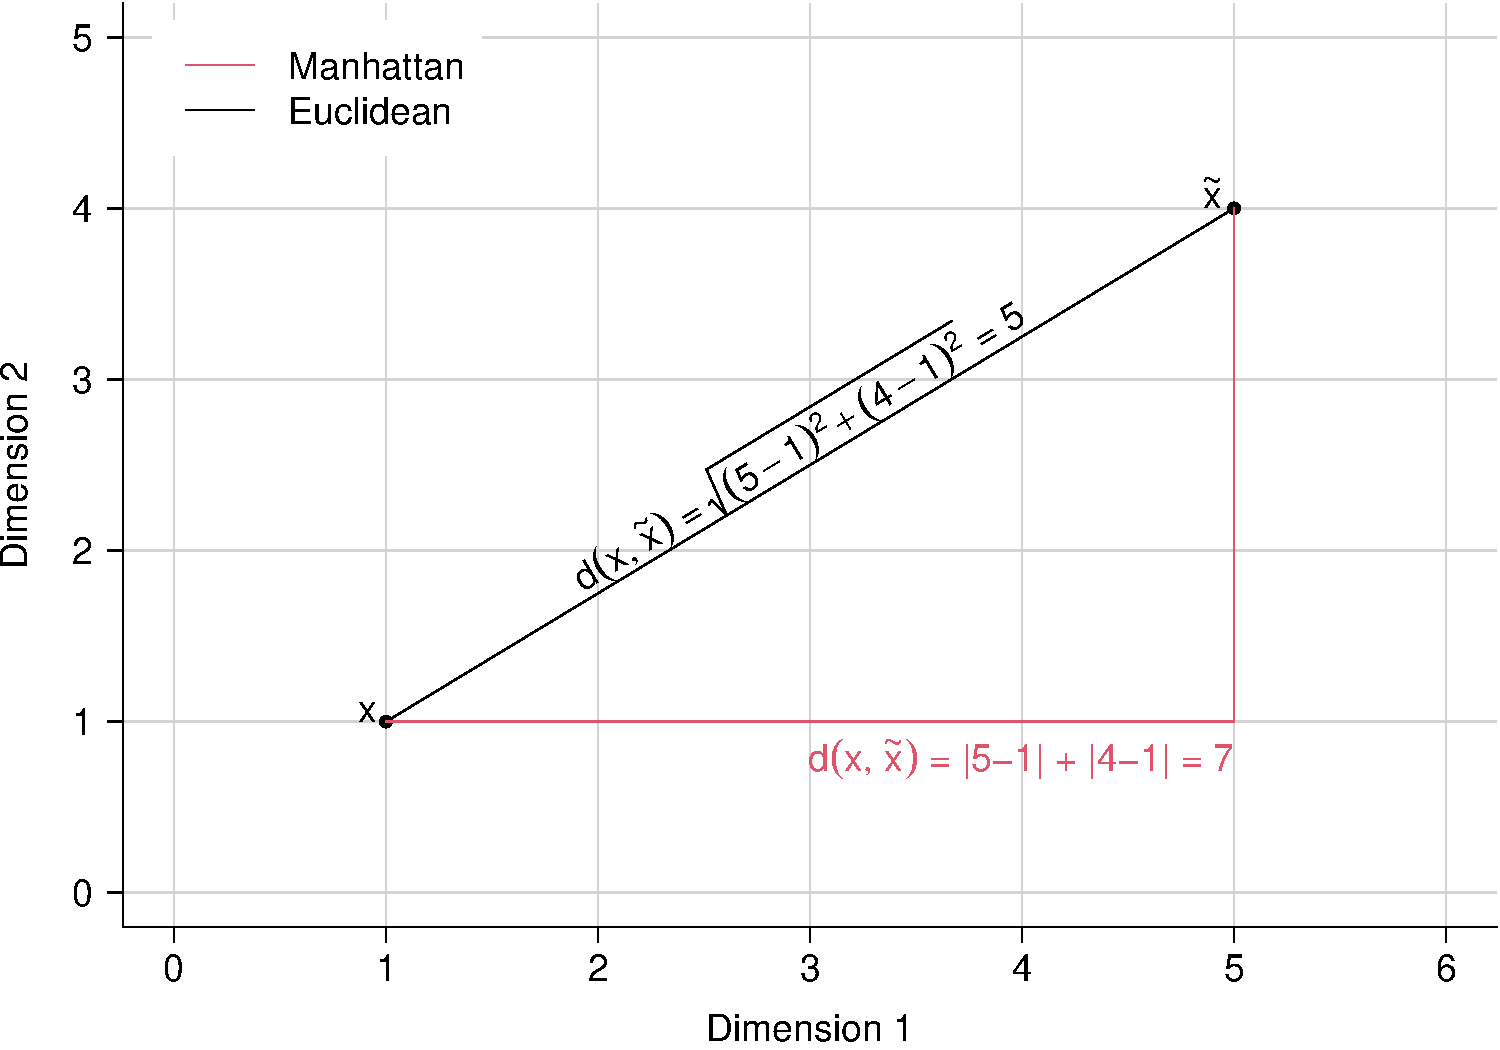
\includegraphics[width=0.9\textwidth,keepaspectratio]{figure/reg_knn_2} 
\end{minipage}
     


\end{vbframe}




\begin{vbframe}{Prediction - Regression}
\begin{footnotesize}
Compute for each point the average output $y$ of the $k$-nearest neighbours in $N_k(\xv)$: 
% \item For regression:
$$
\fxh = \frac{1}{k} \sum_{i: \xi \in N_k(\xv)} \yi \text  { or }  
\fxh = \frac{1}{\sum_{i: \xi \in N_k(\xv)} w^{(i)}} \sum_{i: \xi \in N_k(\xv)} w^{(i)} \yi
$$
with neighbors weighted based on their distance to $\xv$: $w^{(i)} = \frac{1}{d(\xi, \xv)}$
%fig-reg_knn_1_3d.R
\vspace{-0.3cm}
\begin{center}
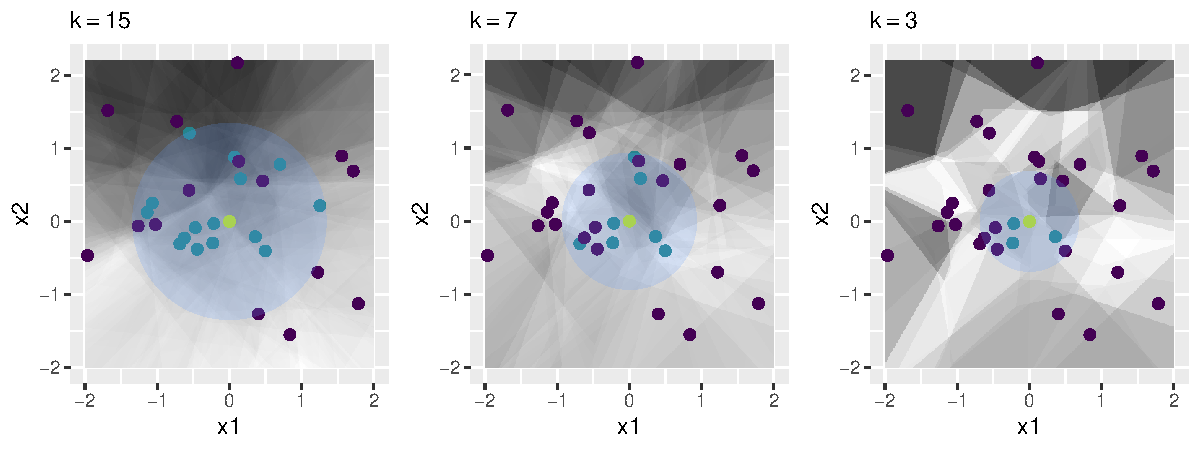
\includegraphics[width=0.65\textwidth,keepaspectratio]{figure/reg_knn_contour}

\vspace{-0.1cm}
%fig-reg_knn_1_contour.R
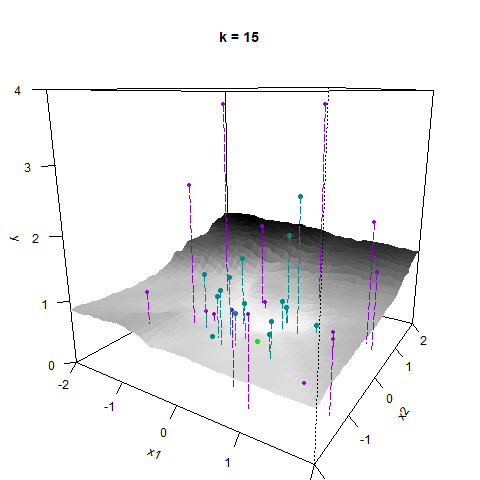
\includegraphics[width=0.25\textwidth]{figure/knn-reg-3d-15.png} 
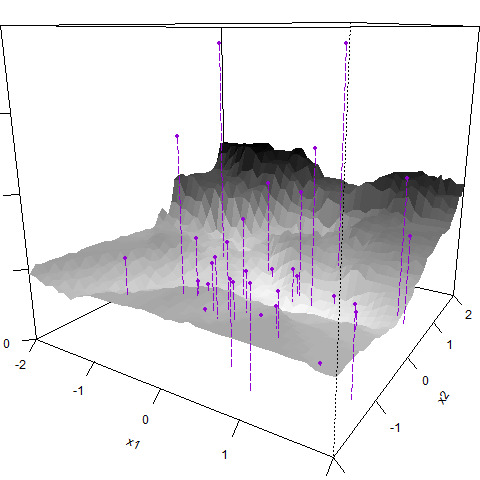
\includegraphics[width=0.25\textwidth]{figure/knn-reg-3d-7.png}
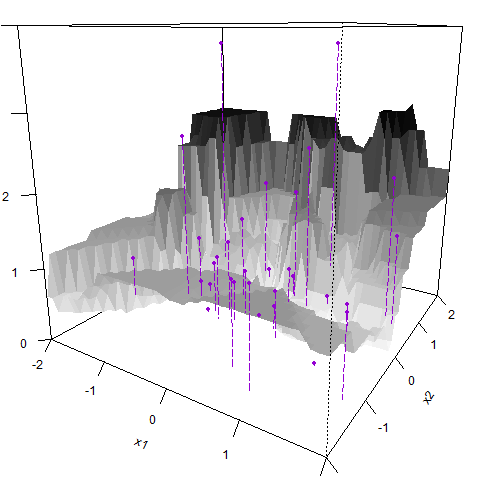
\includegraphics[width=0.25\textwidth]{figure/knn-reg-3d-3.png}
\end{center}

\end{footnotesize}

\end{vbframe}
\begin{vbframe}{Prediction - Classification}

\begin{footnotesize}
For classification in $g$ groups, a majority vote is used: \\
$$
\hxh = \argmax_{\ell \in \gset} \sum_{i: \xi \in N_k(\xv)} \I(\yi = \ell)
$$
And posterior probabilities can be estimated with:
$$
\hat{\pi}_{\ell}(\xv)= \frac{1}{k} \sum_{i: \xi \in N_k(\xv)} \I(\yi = \ell)
$$

\medskip
\begin{columns}[T]
  \begin{column}{0.5\textwidth}
  \centering
\begin{knitrout}\scriptsize
\definecolor{shadecolor}{rgb}{0.969, 0.969, 0.969}\color{fgcolor}

{\centering 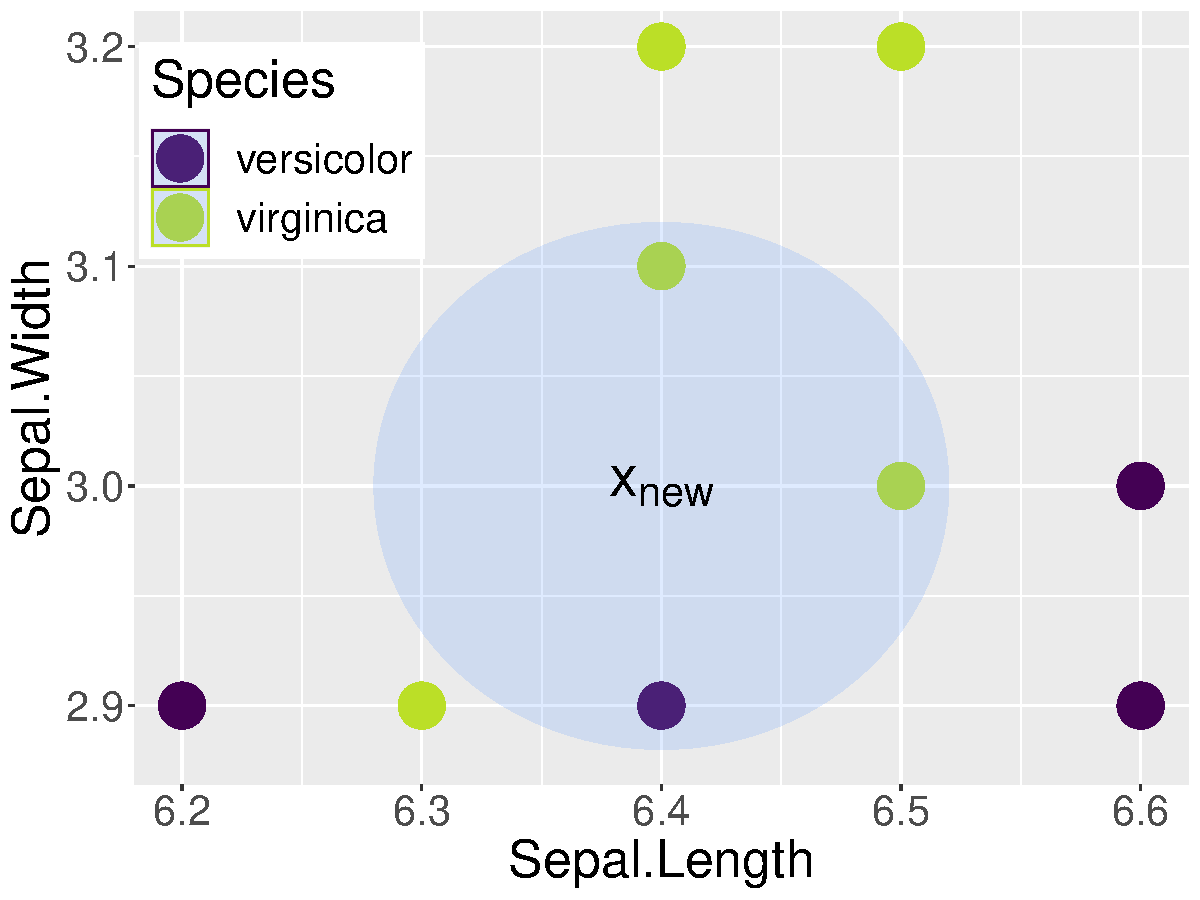
\includegraphics[width=0.7\textwidth, keepaspectratio]{figure/reg_class_knn_1} 

}



\end{knitrout}
  \end{column}
  \begin{column}{0.5\textwidth}
  \centering
\begin{knitrout}\scriptsize
\definecolor{shadecolor}{rgb}{0.969, 0.969, 0.969}\color{fgcolor}
\fontsize{5}{5}\selectfont
\begin{tabular}{l|r|r|l|r}
\hline
  & SL & SW & Species & dist\\
\hline
52 & 6.4 & 3.2 & versicolor & 0.200\\
\hline
59 & 6.6 & 2.9 & versicolor & 0.224\\
\hline
\rowcolor[HTML]{DFECFF}  \textcolor{black}{75} & \textcolor{black}{6.4} & \textcolor{black}{2.9} & \textcolor{black}{versicolor} & \textcolor{black}{0.100}\\
\hline
76 & 6.6 & 3.0 & versicolor & 0.200\\
\hline
98 & 6.2 & 2.9 & versicolor & 0.224\\
\hline
104 & 6.3 & 2.9 & virginica & 0.141\\
\hline
\rowcolor[HTML]{DFECFF}  \textcolor{black}{105} & \textcolor{black}{6.5} & \textcolor{black}{3.0} & \textcolor{black}{virginica} & \textcolor{black}{0.100}\\
\hline
111 & 6.5 & 3.2 & virginica & 0.224\\
\hline
116 & 6.4 & 3.2 & virginica & 0.200\\
\hline
\rowcolor[HTML]{DFECFF}  \textcolor{black}{117} & \textcolor{black}{6.5} & \textcolor{black}{3.0} & \textcolor{black}{virginica} & \textcolor{black}{0.100}\\
\hline
138 & 6.4 & 3.1 & virginica & 0.100\\
\hline
148 & 6.5 & 3.0 & virginica & 0.100\\
\hline
\end{tabular}


\end{knitrout}
  \end{column}
\end{columns}
\medskip
\textbf{Example with subset of iris data ($k = 3$)} \\
$  \hat{\pi}_{setosa}(\xv_{new}) = \frac{0}{3} = 0\% $, 
$  \hat{\pi}_{versicolor}(\xv_{new}) = \frac{1}{3} = 33\% $, 
$  \hat{\pi}_{virginica}(\xv_{new}) = \frac{2}{3} = 67\% $, 
$  \hh(\xv_{new}) = \textit{virginica}$
\end{footnotesize}
\end{vbframe}

\begin{vbframe}{$k$-NN: From small to large $k$}

\begin{knitrout}\scriptsize
\definecolor{shadecolor}{rgb}{0.969, 0.969, 0.969}\color{fgcolor}

{\centering 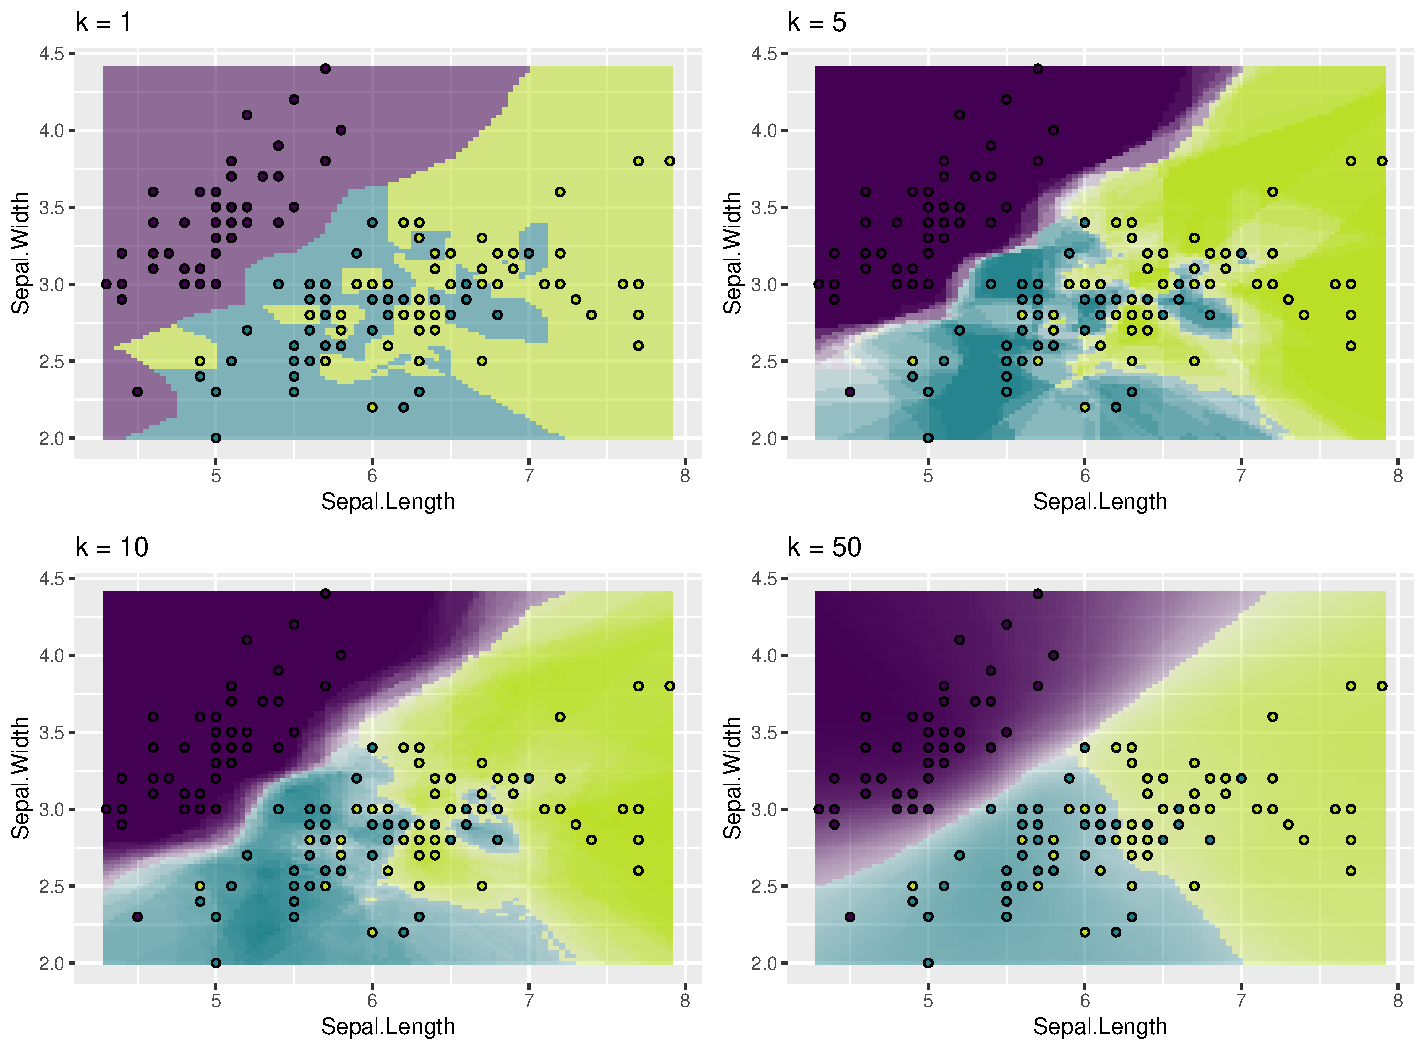
\includegraphics[width=0.95\textwidth,height=7cm]{figure/reg_class_knn_2} 

}



\end{knitrout}
Complex, local model vs smoother, more global model

\end{vbframe}




\begin{vbframe}{$k$-NN Summary}

  \begin{itemize}
  \item $k$-NN is a lazy classifier, it has no real training step, it simply stores the complete data 
    - which are needed during prediction. 
  \item Hence, its parameters are the training data, there is no real compression of information.
  \item As the number of parameters grows with the number of training points, we call 
    $k$-NN a non-parametric model
  \item $k$-NN is not based on any distributional or functional assumption,
    and can, in theory, model data situations of arbitrary complexity.  
  % \item $k$-NN has no optimization step and is a very local model.  
  % \item We cannot simply use least-squares loss on the training data for picking $k$,
    % because we would always pick $k=1$.  
  \item The smaller $k$, the less stable, less smooth and more \enquote{wiggly} the decision
    boundary becomes.  
  \item Accuracy of $k$-NN can be severely degraded by the presence of noisy or irrelevant features,
    or when the feature scales are not consistent with their importance.
  \end{itemize}

% \framebreak
% 
% \lz
% 
% \textbf{Hypothesis Space:} Step functions over tesselations of $\Xspace$.\\
% Hyperparameters: distance measure $d(\cdot,\cdot)$ on $\Xspace$; size of neighborhood $k$.
% 
% \lz
% 
% \textbf{Risk:} Use any loss function for regression or classification.
% 
% \lz
% 
% \textbf{Optimization:} Not applicable/necessary.\\ But: clever look-up methods \& data structures to avoid computing all $n$ distances for generating predictions.

\end{vbframe}

\begin{vbframe}{Standardization and Weights}


\begin{itemize}
  \item \textbf{Standardization:} Features in k-NN are usually standardized or normalized. If two features have values on a very different range, most distances would place a higher importance on the one with a larger range, leading to an imbalanced influence of that feature.
  \item \textbf{Importance:} Sometimes one feature has a higher importance (maybe we know this via domain knowledge). It can now manually be upweighted to reflect this.

$$d^{weighted}_{Euclidean}\left(\xv, \tilde{\xv}\right) = \sqrt{\sumjp w_{j}(x_j- \tilde{x}_j)^2}$$
  
  \item If these weights would have to be learned in a data-driven manner, 
    we could only do this by hyperparameter tuning in k-NN. This is inconvenient,
    and Gaussian processes handle this much better.
\end{itemize}

\end{vbframe}

\begin{vbframe}{Gower distance}
\begin{itemize}
    \item A weighted mean of univ. distances in the j-th feature.
    \item It can handle categoricals, missings, and different ranges.
\end{itemize}


$$d_{gower}(\xv, \tilde{\xv}) = \frac{\sumjp \delta_{x_j,\tilde{x}_j} \cdot d_{gower}(x_j,\tilde{x}_j)}{
\sumjp \delta_{x_j,\tilde{x}_j}}.
$$

\begin{itemize}

  \item \(\delta_{x_j,\tilde{x}_j}\) is 0 or 1. 
  It's 0 if $j$-th feature is \emph{missing} in at least one observation,
  or when the feature is asymmetric binary (where \enquote{1} is more
  important than \enquote{0}) and both values are zero. Otherwise 1.
  \item \(d_{gower}(x_j,\tilde{x}_j)\): 
  For nominals it's 0 if both values are equal and 1 otherwise.
  For integers and reals, it's the absolute difference, divided by range.

\end{itemize}

\framebreak

Example of Gower distance with data on sex and income:

\begin{columns}[T]
  \begin{column}{0.4\textwidth}
\begin{knitrout}\scriptsize
\definecolor{shadecolor}{rgb}{0.969, 0.969, 0.969}\color{fgcolor}\begin{table}[H]
\centering\begingroup\fontsize{10}{12}\selectfont

\begin{tabular}{>{\leavevmode\color{black}}l|>{\leavevmode\color{black}}l|>{\leavevmode\color{black}}r}
\hline
index & sex & salary\\
\hline
1 & m & 2340\\
\hline
2 & w & 2100\\
\hline
3 & NA & 2680\\
\hline
\end{tabular}
\endgroup{}
\end{table}


\end{knitrout}
  \end{column}
  \begin{column}{0.5\textwidth}
    \vspace{0.6cm}
    \fbox{
      $d_{gower}(\xv,\tilde{\xv}) = \frac{\sumjp \delta_{x_j,\tilde{x}_j} \cdot d_{gower}(x_j,\tilde{x}_j)}{
      \sumjp \delta_{x_j,\tilde{x}_j}}
      $}
  \end{column}
\end{columns}

\vfill

$d_{gower}(\xv^{(1)},\xv^{(2)}) = \frac{ 1 \cdot 1 + 1 \cdot \frac{\left| 2340 - 2100 \right|}
{\left| 2680 - 2100 \right|}}{1 + 1} = \frac{1 + \frac{240}{580}}{2} = \frac{1 + 0.414}{2} = 0.707
$

\vfill

$d_{gower}(\xv^{(1)},\xv^{(3)}) = \frac{ 0 \cdot 1 + 1 \cdot \frac{\left| 2340 - 2680 \right|}
{\left| 2680 - 2100 \right|}}{0 + 1} = \frac{0 + \frac{340}{580}}{1} = \frac{0 + 0.586}{1} = 0.586
$

\vfill

$d_{gower}(\xv^{(2)},\xv^{(3)}) = \frac{0 \cdot 1 + 1 \cdot \frac{\left| 2100 - 2680 \right|}
{\left| 2680 - 2100 \right|}}{0 + 1} = \frac{0 + \frac{580}{580}}{1} = \frac{0 + 1.000}{1} = 1
$

\vfill
\end{vbframe}





\endlecture
\end{document}
